% Modern Aspect Ratio
\documentclass[aspectratio=169]{beamer}

\title{Sample Presentation}
\author{VSteinborn}
\date{\today}

\begin{document}

\frame{\titlepage}

\begin{frame}
	\frametitle{Simple 2D Graph \cite{dr_trefor_bazett_how_2022}}

	\begin{center}
		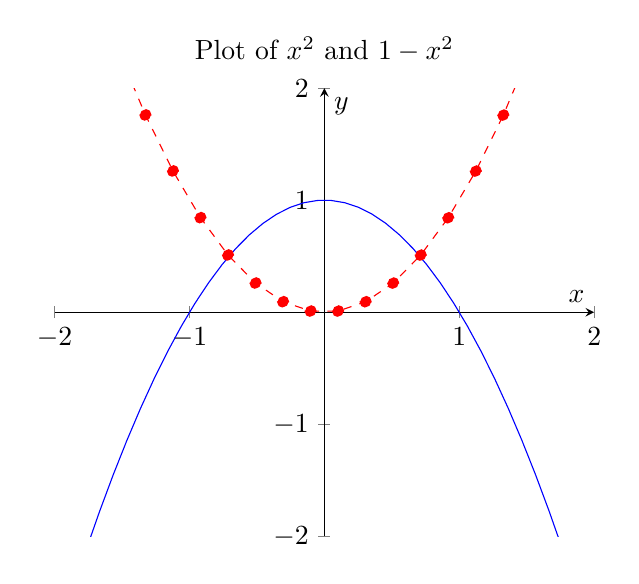
\begin{tikzpicture}
			\begin{axis}[
				xmin=-2, xmax=2, ymin=-2, ymax=2,
				axis lines = middle,
				xlabel=$x$, ylabel=$y$,
				title={Plot of $x^2$ and $1-x^2$},
				]
				\addplot[
					color=red, dashed, mark=*, samples=50
					]{x^2};
				\addplot[
					color=blue, samples=100
					]{1-x^2};
			\end{axis}
		\end{tikzpicture}
	\end{center}
\end{frame}

\begin{frame}
	\frametitle{Annotated 2D Graph \cite{dr_trefor_bazett_how_2022}}

	\begin{columns}
		\column{0.3\textwidth}
		\begin{itemize}
			\item Currently using the Metropolis \cite{matthias_vogelgesang_ctan_2017} theme
		\end{itemize}

		{\metroset{block=fill}
		\begin{block}{Key Point 1}
			Block content
		\end{block}}

		\begin{block}{Key Point 2}
			Block content
		\end{block}

		\begin{exampleblock}{Custom Example Block}
			Block content
		\end{exampleblock}

		\column{0.7\textwidth}
		\begin{center}
			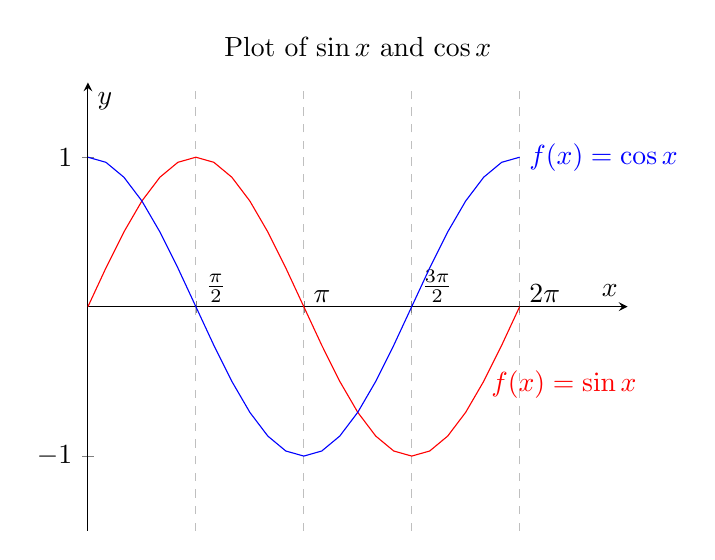
\begin{tikzpicture}
				\begin{axis}[ clip=false,
					xmin=0, xmax=2.5*pi, ymin=-1.5, ymax=1.5,
					axis lines=middle,
					xtick ={0, pi/2, pi, 3*pi/2, 2*pi},
					xticklabels={$0$, $\frac{\pi}{2}$, $\pi$, $\frac{3\pi}{2}$, $2\pi$},
					xticklabel style={anchor=south west},
					xmajorgrids=true,
					grid style=dashed,
					xlabel=$x$, ylabel=$y$,
					title={Plot of $\sin x $ and $\cos x$},
					]
					\addplot[
						domain=0:2*pi,red
						]{sin(deg(x))}
					node[right,pos=0.9]{$f(x)=\sin x$};
					\addplot[
						domain=0:2*pi,blue
						]{cos(deg(x))}
					node[right,pos=1]{$f(x)=\cos x$};
				\end{axis}
			\end{tikzpicture}
		\end{center}

		
	\end{columns}
\end{frame}

\begin{frame}[standout]
	Questions?
\end{frame}

\begin{frame}[allowframebreaks]{References}

	\bibliography{sample_beamer}
	\bibliographystyle{abbrv}
  
\end{frame}

\end{document}